\documentclass[10pt,landscape,a4paper]{article}
\usepackage{multicol}
\usepackage[landscape]{geometry}
\usepackage{hyperref}
\usepackage[utf8]{inputenc}
\usepackage{minted}
\usepackage{graphicx}


\geometry{top=0.5cm,left=0.5cm,right=0.5cm,bottom=0.5cm}

% Turn off header and footer
\pagestyle{empty}
 
% Redefine section commands to use less space
\makeatletter
\renewcommand{\section}{\@startsection{section}{1}{0mm}%
                                {-1ex plus -.5ex minus -.2ex}%
                                {0.5ex plus .2ex}%x
                                {\normalfont\large\bfseries}}
\renewcommand{\subsection}{\@startsection{subsection}{2}{0mm}%
                                {-1explus -.5ex minus -.2ex}%
                                {0.5ex plus .2ex}%
                                {\normalfont\small\bfseries}}
\renewcommand{\subsubsection}{\@startsection{subsubsection}{3}{0mm}%
                                {-1ex plus -.5ex minus -.2ex}%
                                {1ex plus .2ex}%
                                {\normalfont\footnotesize\bfseries}}
\makeatother

% Don't print section numbers
\setcounter{secnumdepth}{0}

\setlength{\parindent}{0pt}
\setlength{\parskip}{0pt plus 0.5ex}

\newcommand{\java}[1]{\mintinline{java}{#1}}


% -----------------------------------------------------------------------

\begin{document}

\footnotesize
\begin{multicols*}{3}


% multicol parameters
% These lengths are set only within the two main columns
%\setlength{\columnseprule}{0.25pt}
\setlength{\premulticols}{1pt}
\setlength{\postmulticols}{1pt}
\setlength{\multicolsep}{1pt}
\setlength{\columnsep}{2pt}


\section{Primitive Datentypen}
Alle signed\\
\begin{tabular}{lll}
 boolean & Boolescher Wert & true,false \\
 \hline
 char & UTF16, 16Bit & 'a', 'B', '0', 'ë' etc. \\
 \hline
 byte & 8 Bit  & -128 bis 127 \\
short & 16 Bit & 32'768 bis 32'767\\
int & 32 Bit &  -2$^{31}$ bis 2$^{31}$ -1\\
long & 64 Bit  & -2$^{63}$ bis 2$^{63}$ -1 , 1l (l Suffix, zwingend)\\
\hline
float & 32 Bit & 0.1f, 2e4f (2 * 10$^4$) (f Suffix, zwingend)\\
double & 64 Bit  & 0.1, 2e4 (d Suffix, nicht zwingend)
\end{tabular}
Float comparison: \java{Math.abs(a - b) < 1e-8} sonst nummerische Fehler, 
1/0: \java{ArithmeticException},
0/0.0: \java{NaN},
1/0.0: \java{Double.POSITIVE_INFINITY},
-1/0.0: \java{Double.NEGATIVE_INFINITY}

\subsection{Casts}
\begin{multicols}{2}
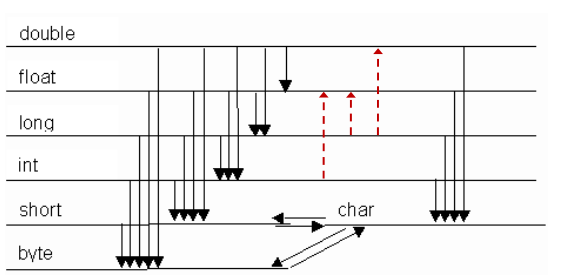
\includegraphics[width=\columnwidth]{casts.png}
\vfill\null
\columnbreak
schwarz: explizit, \textcolor{red}{implizit (ggf. Genauigkeitsverlust)}, andere implizit\\
Ganzzahl zu Ganzzahl(nur untere Bits): \java{(byte)0x1234}$\rightarrow$0x34 
Gleitkommazahl zu Ganzzahl$\rightarrow$wird abgeschnitten 3.7$\rightarrow$3
\end{multicols}

%\subsection{Initialisierung}
%\textbf{Lokale Variablen/innerhalb von Methoden:} zwingend initialisieren \textbf{Instanz/Klassen-Variablen:} nicht zwingend, sonst Default-Wert

\section{Referenzielle Datentypen}

\subsection{Array}
%\textbf{Erzeugung 1. Ebene} \java{int [] [] termine = new int [31] [];}\\
%\textbf{Erzeugung 2. Ebene} \java{termine [1] = new int [24];}\\
%\textbf{Erzeugung zusammen} \java{int [][] termine = new int [31] [24]}
%\textbf{Länge erste Ebene} \java{termine.length}\\
%\textbf{Länge zweite Ebene bei Index 0} \java{termine [0].length}\\
\java{Arrays.equals(array1, array2)}\\
\java{Arrays.deepEquals(array1, array2)} für mehrdimensionale

\subsection{Enum}
\begin{minted}{Java}
public enum Weekday{
Monday(true), Tuesday(true), ...
private boolean workday;
/*Nur privater Konstruktor, implizit*/
Weekday(boolean workDay){this.workDay = workDay;}
public boolean isWorkDay(){return WorkDay;}}
\end{minted}

\begin{minted}{Java}
enum Snafu{DISCORDIA, ERIS}
Snafu goettin = Snafu.ERIS;
\end{minted}

%\section{Operatoren}
%Unäre Operatoren (z.B. \java{a++}) vor binären\\
%Linksassoziativ\\
%\java{x = a ? b : c}:  wenn ? dann : sonst

\section{Selektionen/Schlaufen}
\java{for (String s : array|arrayList){...}}\\
\java{switch (int|char|String|...){case wert1: break;}default:}

%\section{Methoden}
%Signatur = Methodenname + Parametertypen\\
%Methodenaufruf$\rightarrow$Methode wird auf Stack geladen\\
%Java nur Call by Value!
%
%\subsection{Overloading}
%Mehrere Methoden mit gleichem Namen, unterschiedliche Parametertypen
%
%\subsection{Overriding}
%\java{@Override}
%Subklasse implementiert gleiche Methode$\rightarrow$überschreibt sie,
%Signatur muss gleich sein
%\java{final} Methoden können nicht überschrieben werden
%\subsection{Dynamic Dispatch}
%Bei Aufruf nicht privater Instanzmethoden:\\
%\textcolor{red}{Statischer Typ: zur Compile-Zeit}, \textcolor{blue}{Dynamischer Typ: zur Laufzeit}\\
%\textcolor{red}{Vehicle} vehicle = new \textcolor{blue}{Car}();
%\begin{minted}{Java}
%Car c = new Car();
%Vehicle v = c; 
%v.print(); ((Vehicle)c).print(); //bei beiden: Methode von Car
%\end{minted}

\section{Overloading/Overriding}
\java{super.methodenname();} $\rightarrow$ überschriebene Methode aufrufen,
Verweise innerhalb  \java{super}Methode, wenn überschrieben, automatisch Aufruf der überschriebenen\\
Test ob dynamischer Typ auf statischer passt: reference \java{instanceof} TypeName\\
Variablenwerte werden nicht überschrieben!

\section{Klassen}
\begin{minted}{Java}
abstract class Vehicle {
abstract void report();
void print() {...}}
\end{minted}

von \java{final} Klassen kann nicht geerbt werden, Alle Methoden auch automatisch \java{final}

\section{Interface}
Methoden implizit public \& abstract\\
nur Konstanten erlaubt (keine Variablen)\\
\java{default}-Methoden: Können überschrieben werden, sonst Default-Implementierung, \java{static} unterstützt, Member von \java{Object}\\
Mehrere Default-Methoden mit gleicher Signatur, Adressierung: \java{nameInterface.super.methodenName();}

%\section{Exception}
%\begin{minted}{java}
%class MyException extends Exception {
%  MyException(String message) {
%    super(message);
%  }
%}
%public String clip(String s) throws MyException {
%  throw new MyException("bla");
%}
%try {
%  s = clip(s);
%} catch (MyException | OtherException e) {
%  e.getMessage();
%  e.printStackTrace();
%}finally{}
%\end{minted}

%\java{RuntimeException}, \java{Error}$\rightarrow$unchecked, keine Behandlung\\
%\java{IllegalArgumentException} an der Prüfung einsetzen


\section{Varia}
\subsection{Zugriffskontrolle}
\textbf{public: }Alle Klassen, \textbf{protected: }Package + Sub-Klassen,
\textbf{(keines): }selbes Package, \textbf{private: }eigene Klasse

\subsection{Packages}
\java{package p1;} \java{package p1.sub;}\\
\java{import p1.*; //Alle public Klassen, p1.sub nicht}\\
Klassenvariablen direkt benutzen: \java{import static java.lang.System.out;}

\subsection{Scanner}
\java{Scanner scanner = new Scanner(System.in);}

\subsection{Primzahlen}
\begin{minted}{Java}
public boolean isPrime(long number) {
if (number <= 1) {
throw new IllegalArgumentException("number must be > 1");}
for (long x = 2; x <= Math.sqrt(number); x++) {
if (number % x == 0) { return false; }}
return true;}
\end{minted}

\subsection{Kleinster Wert}
\begin{minted}{Java}
 double min = Double.MAX_VALUE;
 TreeNode smallest = null;
 for (TreeNode node: trees) {
 if (node.getFrequency() < min) {
 min = node.getFrequency();
 smallest = node;}
\end{minted}

\subsection{Permutation}
\begin{minted}{Java}
 public static <T> void generate
 (List<T> permutation, Set<T> rest, PermutationEater<T> eater) {
  if(rest.isEmpty())
    eater.eat(permutation);                                            
  else
   for(T element: rest) {
   permutation.add(element);
   Set<T> restCopy = new HashSet<>(rest);
   restCopy.remove(element);
   generate(permutation, restCopy, eater);
   permutation.remove(element);}}}
\end{minted}

\subsection{Potenzmenge generieren}
\begin{minted}{Java}
static <T> Set<Set<T>> powerSet(List<T> elements) {
if (elements.size() == 0) {
	Set<Set<T>> empty = new HashSet<>();
	empty.add(new HashSet<>());
	return empty;}
List<T> remaining = new ArrayList<>(elements);
T current = remaining.remove(0);
Set<Set<T>> result = new HashSet<>();
for (Set<T> set : powerSet(remaining)) {
    result.add(set);
	Set<T> augmentedSet = new HashSet<>(set);
	augmentedSet.add(current);
	result.add(augmentedSet);}
return result;}
\end{minted}

\subsection{Verknüpfungen}
\begin{minted}{Java}
boolean isLinked(Person from, Person to) { 
return isLinked(from, to, new HashSet<>()); }

boolean isLinked(Person from, Person to, Set visited) { 
if (from == to) { return true; } 
if (visited.contains(from)) { return false; } 
visited.add(from); 
for (Person other : from.getKnownPeople()) 
{ if (isLinked(other, to, visited)) {
return true; } 
} return false; }
\end{minted}

\section{Objektmethoden}
\subsection{Equals}
\begin{minted}{Java}
@Override
public boolean equals(Object obj) {
if (obj == null) { 
return false;} 
if (getClass() != obj.getClass()) {
return false;} //von gleicher Klasse produziert?
Person other = (Person)obj;
return Objects.equals(firstName, other.firstName) && 
Objects.equals(lastName, other.lastName);
}}//Objects: null=null -> true, sonst equals-Methode
\end{minted}

\subsection{CompareTo}
$<$ 0: this ist kleiner als other
, $>$ 0: this ist grösser als other
, 0: this ist gleich other
\begin{minted}{Java}
class Person implements Comparable<Person> {
private String firstName, lastName;
@Override
public int compareTo(Person other) {
int result = lastName.compareTo(other.lastName);
if (result == 0) {
result = firstName.compareTo(other.firstName);
} return result; }}
\end{minted}
\subsection{clone}
\begin{minted}{Java}
class Person implements Cloneable {
@Override
public Person clone() {
return new Person(firstName, lastName); }}
// (Person)super.clone () CloneNotSupportedException
\end{minted}

%\subsection{Hash}
%0\begin{minted}{Java}
%@Override
%public int hashCode(){
%return firstName.hashCode() + 31 * lastName.hashCode();
%}
%\end{minted}

\section{Java Collections}

%\begin{tabular}{llll}
%& Finden & Einfügen & Löschen\\
%\hline 
%ArrayList & langsam & sehr schnell am Ende & langsam\\
%LinkedList & langsam & sehr schnell am Ende & Ende: sehr schnell\\
%HashSet & sehr schnell & sehr schnell & sehr schnell\\
%HashMap & sehr schnell & sehr schnell & sehr schnell\\
%TreeSet & \textcolor{yellow}{schnell} & schnell & schnell\\
%TreeMap & schnell & schnell & schnell\\
%\end{tabular}

\begin{multicols}{2}
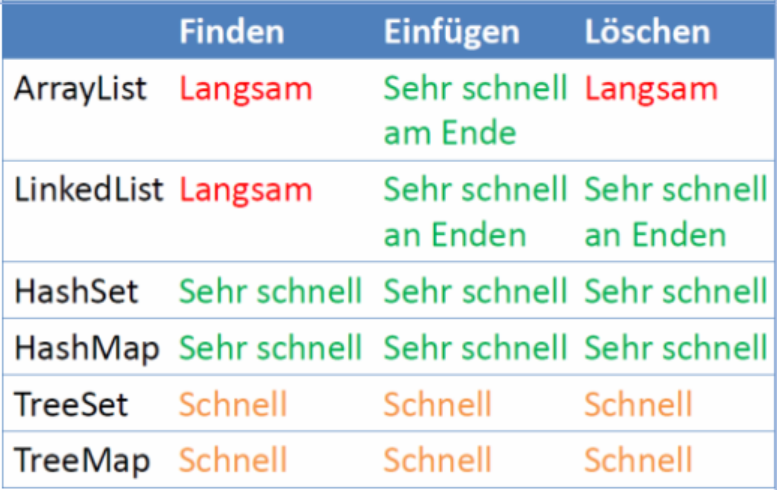
\includegraphics[width=\columnwidth]{collections1.PNG}
\vfill\null
\columnbreak
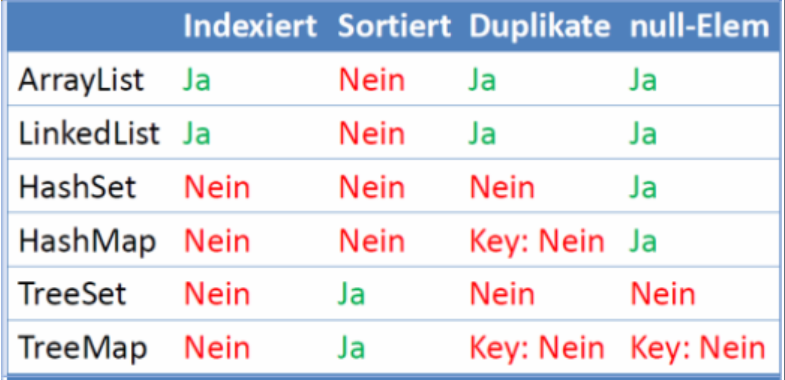
\includegraphics[width=\columnwidth]{collections2.PNG}
\end{multicols}

\subsection{Methoden}
\textbf{Collection}:\java{size()}, \java{toArray()}, \java{clear()}, \java{isEmpty()}\\ 
$\rightarrow$\textbf{List}: \java{set(index)}, \java{get(index)}\\
$\rightarrow$\textbf{Set}: \java{implements Comparable<T>}, \java{add(obj)}\\
\textbf{Maps}: wie Sets, \java{containsKey(Obj key)}, \java{containsValue}\java{(Obj value)}, \java{put(K key, V value)}, \java{Collection<V> values()}

\subsection{Iteration}
\begin{minted}{Java}
Iterator<String> it = stringList.iterator();
while (it.hasNext()) {
String elem = it.next();
if (elem.equals("...")) {
it.remove();} //geht nur bei richtigem Iterator
\end{minted}

Iterator geht nur mit Sets, Lists
| Alternativen für \java{HashMap}

\begin{minted}{Java}
for (int i : hashMap.keySet()){
hashMap.get(i);}
\end{minted}

\begin{minted}{Java}
for (Map.Entry<Character, Double> entry: map.entrySet()) {
 entry.getValue(), entry.getKey()}
\end{minted}

\subsection{Comparator}
\java{Collections.sort(List<T> list);} \\
aufsteigend, Alle Elemente: Comparable\\
\java{Collections.sort(List<T> list, Comparator<T> comparator);}\\
\begin{minted}{Java}
class MyComparator implements Comparator<Person>{
@Override
public int compare(Person p1, Person p2){}}
\end{minted}

\section{Generics}
\subsection{Klasse}
\java{Node<String> stringNode = new Node<>();}
\begin{minted}{Java}
class Pair <T, U> {
private final T first;
private final U second;}
\end{minted}
T muss von Klasse Person und weiterer erben/implementieren:\\
\java{class Node<T extends Person & weitere> {...}}\\
Nodes müssen sortiert werden können:\\
\java{class Node<T extends Comparable<T>>}
\subsection{Methode}
\java{public <T> T majority(T x, T y, T z){...}}\\
Bei generischen Klassen$\rightarrow$\java{<T>} bei Methode nicht angeben!\\ \\
Gewisse Klasse oder Sub-Klasse:\\
\java{Node<? extends Person>node;}\\
Gewisse Klasse oder Super-Klasse:\\
\java{Node <? super Person>node;}

\section{Methodenreferenzen}
Passen auf Funktionsschnittstellen \java{@FunctionalInterface} (genau 1 abstrakte Methode)

\java{this::compare}: im selben Objekt\\
\java{other::compare}: in Objekt other\\
\java{MyClass::compare}: statische in Klasse MyClass\\
\java{MyClass::new}: Konstruktor der Klasse MyClass

\section{Lambda}
weglassen (wird berechnet): Rückgabetyp, Typen der Parameter, \{\} des Body\\
\java{(p1, p2) -> Integer.compare(p1.getAge(), p2.getAge())}\\
() weglassen, wenn nur ein Parameter\\
\java{p -> p.getAge() >= 18}\\
Zugriff in Lambdas auf lokale Variablen?$\rightarrow$Variablen automatisch \java{final} (auch ohne Deklaration)

%\section{Geschachtelte Klassen}
%\subsection{Innere Klassen}
%\begin{minted}{Java}
%Polygon myPolygon = new Polygon();
%Polygon.Point point = myPolygon.new Point (1, 2);
%\end{minted}
%
%Statisch:
%\java{Polygon.Point point = new Polygon.Point();}
%
%\subsection{Lokale Klasse}
%innerhalb Methode
%
%\subsubsection{Anonyme innere Klasse}
%\begin{minted}{Java}
%people.sort(
%New Comparator<Person>(){
%@Override
%public int compare...})
%\end{minted}

\section{Stream API}

%{a) Alle unterschiedlichen Vornamen weiblicher Personen mit maximal 3 Buchstaben
%b) Durchschnittsalter aller männlicher Personen
%c) Minimalalter aller Personen
%d) Top 10 Verdiener (Jahreseinkommen)
%e) Durchschnittsalter pro Ort (Gruppierung mittels Collector)
%
%\begin{minted}{Java}
%people.stream()//a
%.filter(p -> p.getGender() == Gender.FEMALE)
%.map(Person::getFirstName)
%.filter(n -> n.length() <= 3)
%.distinct()
%.forEach(System.out::println);
%people.stream()//b
%.filter(p -> p.getGender() == Gender.MALE)
%.mapToInt(Person::getAge)
%.average()
%.getAsDouble());
%//c
%people.stream().mapToInt(Person::getAge).min().getAsInt()
%stream()//d
%.sorted(Comparator.comparing(Person::getSalary).reversed())
%.limit(10)
%.map(p -> p.getFirstName() + " " + p.getLastName() + " "
%+ p.getCity())
%.forEach(System.out::println);
%//e
%stream()
%.collect(Collectors.groupingBy(Person::getCity, 
%Collectors.averagingInt(Person::getAge)))
%.forEach((city, age) -> System.out.println(city + " " + age));
%\end{minted}

\subsection{Zwischenoperationen}
\begin{minted}{Java}
people
 .stream()
 //Filtern mit Lamda/Predicate-Fktobj
 .filter(p -> p.getAge() >=18)
 //Projizieren nur Lambda oder prim. Datentyp
 .map(p ->  p.getLastName())
 .mapToInt/mapToLong/mapToDouble(Function)
 //weitere
 .sorted([Comparator])
 .distinct()//gemäss equals
 .limit(long n)
 .skip(long n)
\end{minted}

\subsection{Terminaloptionen}
\begin{minted}{Java}
 .forEach(System.out::print);
 .forEachOrdered(Sys...);//erhält Reihenfolge
 .count();
 .min([Comp.]);|.max([Comp.]);
 .average();, sum(); //Int, Long, Double
 .findAny();, findFirst(); //irgend, 1.
 .reduce();
 .toArray();
\end{minted}

\java{sum()}:
\begin{minted}{Java}
people.stream()
 .mapToInt(p -> p.getAge())
 .reduce((age1, age2) -> age1 + age2);
\end{minted}

\java{average()}, \java{min()}, \java{max()} lieferen Optional-Werte 
$\rightarrow$\java{OptionalDouble}, \java{OptionalLong}, \java{OptionalInt}

\java{if (averageAge.isPresent())}\\ 
\java{averageAge.ifPresent(System.out::println)}

\java{allMatch(), anyMatch(), noneMatch()}:
\begin{minted}{Java}
boolean adultsOnly =
 people.stream()
  .allMatch(p -> p.getAge() >= 18);
\end{minted}

unendliche Quellen:
\begin{minted}{Java}
Randon random = new Random();
Stream.generate(random::nextInt);
\end{minted}

\java{Intstream.iterate(0, i -> i + 1)}

Rückumwandlung in Collection:
\begin{minted}{Java}
Map<String, Integer> totalAgeByCity =
people.stream()
.collect(Collectors.groupingBy(Person::getCity,
Collectors.summingInt(Person::getAge)));
\end{minted}

\section{Input/Output}
Byte Streams: 8-Bit Daten, \java{InputStream},\java{OutputStream}\\
\begin{minted}{Java}
try (FileInputStream in = new FileInputStream("...")){
} catch (FileNotFoundException e){
} catch (IOException e) {} //Fehler beim Lesen
\end{minted}
Character Stream: 16-Bit (UTF-16), \java{Reader}, \java{Writer}

\begin{minted}{Java}
try (FileReader reader = new FileReader("quotes.txt")){
int value = reader.read(); //zwingend int, da -1 bei Ende
while (value >= 0) {
char c = (char)value;
//use character
value = reader.read();}}
\end{minted}

\begin{minted}{Java}
try (FileWriter writer = new FileWriter("test.txt", true)){
writer.write("Hello!");
writer.write('\n');}
\end{minted}

\begin{minted}{Java}
BufferedReader bufferedReader = new BufferedReader(fileReader);
String line = bufferedReader.readLine();
\end{minted}

\subsection{Serialisieren}
\java{Person implements Serializable}

ausschliessen von Serialisierung: \java{private transient int age;}

\begin{minted}{Java}
try (ObjectOutputStream stream = new ObjectOutputStream(
new FileOutputStream("serial.bin"))) {
stream.writeObject(person);}
\end{minted}

\begin{minted}
try (ObjectInputStream stream = new ObjectInputStream(
new FileInputStream("serial.bin"))) {
Person p = (Person)stream.readObject();…}
//Version geprüft, InvalidCastException
\end{minted}

\section{Regex}
Uhrzeit: 
\java{if(Pattern.matches("[0-2][0-9]:[0-5][0-9]", myText))}
\begin{minted}{Java}
(?<HOURS>[0-2]?[0-9]):(?<MINUTES>[0-5][0-9])
String hoursPart = matcher.group("HOURS"|1);
.*\n[A-Z]*-([0-9]*).*//CH-8640
\end{minted}
\java{Integer.parseInt(line.substring(0, 3)//3 exkl.}

\section{JUnit}

\begin{tabular}{ll}
\java{assertEquals(expected, actual)}       &   actual «equals» expected \\
\java{ssertNotEquals(expected, actual)}     &   !(actual «equals» expected)\\
\java{assertSame(expected, actual)}         &   Referenzvergleich\\
\java{assertNotSame(expected, actual)}      &   !Referenzvergleich\\
\java{assertTrue(condition)}                &   condition\\
\java{assertFalse(condition)}               &   !condition\\
\java{assertNull(value)}                    &   value == null\\
\java{assertNotNull(value)}                 &   value != null\\
\java{fail()}                               &   Immer verletzt
\end{tabular}

\begin{minted}{Java}
@Test
void testUnderflow() {
assertThrows(StackException.class, () -> {
Stack s = new Stack<String>(10);
s.pop();});}
\end{minted}

\end{multicols*}
\end{document}